\documentclass[12pt,a4paper]{scrartcl} 
\usepackage[utf8]{inputenc}
\usepackage[english,russian]{babel}
\usepackage{indentfirst}
\usepackage{misccorr}
\usepackage{graphicx}
\usepackage{indentfirst}
\usepackage{amsmath}
\begin{document}
	\begin{titlepage}
		\begin{center}
			\large
			МИНИСТЕРСТВО НАУКИ И ВЫСШЕГО ОБРАЗОВАНИЯ РОССИЙСКОЙ ФЕДЕРАЦИИ
			
			Федеральное государственное бюджетное образовательное учреждение высшего образования
			
			\textbf{АДЫГЕЙСКИЙ ГОСУДАРСТВЕННЫЙ УНИВЕРСИТЕТ}
			\vspace{0.25cm}
			
			Инженерно-физический факультет
			
			Кафедра автоматизированных систем обработки информации и управления
			\vfill

			\vfill
			
			\textsc{Отчет по практике}\\[5mm]
			
			{\LARGE Программаная реализация численного метода \LARGE{ Нахождение обратной матрицы методом исключения неизвестных Гаусса.}}
			\bigskip
			
			2 курс, группа 2ИВТ
		\end{center}
		\vfill
		
		\newlength{\ML}
		\settowidth{\ML}{«\underline{\hspace{0.7cm}}» \underline{\hspace{2cm}}}
		\hfill\begin{minipage}{0.5\textwidth}
			Выполнил:\\
			\underline{\hspace{\ML}} Ю.\,А.~Береснев\\
			«\underline{\hspace{0.7cm}}» \underline{\hspace{2cm}} 2021 г.
		\end{minipage}%
		\bigskip
		
		\hfill\begin{minipage}{0.5\textwidth}
			Руководитель:\\
			\underline{\hspace{\ML}} С.\,В.~Теплоухов\\
			«\underline{\hspace{0.7cm}}» \underline{\hspace{2cm}} 2021 г.
		\end{minipage}%
		\vfill
		
		\begin{center}
			Майкоп, 2021 г.
		\end{center}
	\end{titlepage}
	
% Содержание
\section{Введение}
\label{sec:intro}


\subsection{Цель работы}
Целью данной работы является вычисление матрицы обратной заданной. 

\subsection{Теория}
Нахождение обратной матрицы методом исключения неизвестных Гаусса. Первый шаг для нахождения обратной матрицы методом исключения неизвестных Гаусса - приписать к матрице A единичную матрицу того же порядка, отделив их вертикальной чертой. Мы получим сдвоенную матрицу $(A|E)$.Умножим обе части этой матрицы на  $A^-^1$. Тогда получим $(A\cdot A^-^1|E\cdot A^-^1)$, но $A\cdot A^-^1=E$ и $E\cdot A^-^1=A^-^1$.


\section{Ход работы}
\subsection{Код программы}
\begin{verbatim}
#include <conio.h>
#include <iostream>
#include <math.h>
using namespace std;
int opr(double** a, int n) { 
    if (n == 1)
        return a[0][0];
    else if (n == 2)
        return a[0][0] * a[1][1] - a[0][1] * a[1][0];
    else {
        double d = 0;
        for (int k = 0; k < n; k++) {
            double** m = new double* [n - 1];
            for (int i = 0; i < n - 1; i++) {
                m[i] = new double[n - 1];
            }
            for (int i = 1; i < n; i++) {
                int t = 0;
                for (int j = 0; j < n; j++) {
                    if (j == k)
                        continue;
                    m[i - 1][t] = a[i][j];
                    t++;
                }
            }
            d += pow(-1, k + 2) * a[0][k] * opr(m, n - 1);
        }
        return d;
    }
}
void obr(double** O, int n)
{
    double temp;
    double** E = new double* [n];

    for (int i = 0; i < n; i++)
        E[i] = new double[n];

    for (int i = 0; i < n; i++)
        for (int j = 0; j < n; j++)
        {
            if (i == j) E[i][j] = 1.0;
            else E[i][j] = 0.0;
        }

    for (int k = 0; k < n; k++)
    {
        temp = O[k][k];

        for (int j = 0; j < n; j++)
        {
            O[k][j] /= temp;
            E[k][j] /= temp;
        }

        for (int i = k + 1; i < n; i++)
        {
            temp = O[i][k];

            for (int j = 0; j < n; j++)
            {
                O[i][j] -= O[k][j] * temp;
                E[i][j] -= E[k][j] * temp;
            }
        }
    }

    for (int k = n - 1; k > 0; k--)
    {
        for (int i = k - 1; i >= 0; i--)
        {
            temp = O[i][k];

            for (int j = 0; j < n; j++)
            {
                O[i][j] -= O[k][j] * temp;
                E[i][j] -= E[k][j] * temp;
            }
        }
    }
    for (int i = 0; i < n; i++)
        for (int j = 0; j < n; j++)
            O[i][j] = E[i][j];
}
int main()
{
    setlocale(LC_ALL, "Russian");
    int n;
    cout << "Укажите размерность квадратной матрицы:" << endl << "n=";
    cin >> n;
    double** A = new double* [n];
    cout << "Введите элементы матрицы:" << endl;
    for (int i = 0; i < n; i++) {
        A[i] = new  double[n];
        for (int j = 0; j < n; j++) {
            cout << "A[" << i << "][" << j << "]=";
            cin >> A[i][j];
        }
    }
    if (n < 1) cout << "Определитель вычислить невозможно и обратной матрицы не существует";
    else
    {
        cout << "Определитель для заданной матрицы = " << opr(A, n) << endl;
        if (opr(A, n) == 0) cout << "Матрица вырожденная и обратной матрицы для неё не существует";
        else {
            obr(A, n);
            cout << "Обратная матрица для заданной:" << endl;
            for (int i = 0; i < n; i++) {
                for (int j = 0; j < n; j++) {
                    cout << A[i][j] << "  ";
                } cout << endl;
            }
        }
    }
    _getch();
    return 0;
}
\end{verbatim}

\begin{figure}[!h]
	\centering
	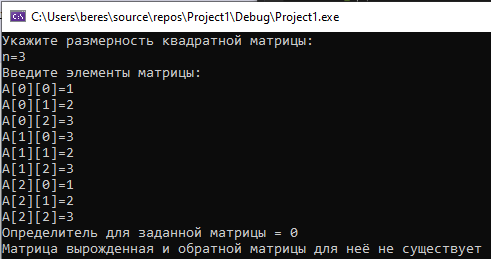
\includegraphics[width=0.7\textwidth]{Рисунок.PNG}
	\caption{Окно программы с вырожденной матрицей}\label{fig:par}
\end{figure}
\begin{figure}[!h]
	\centering
	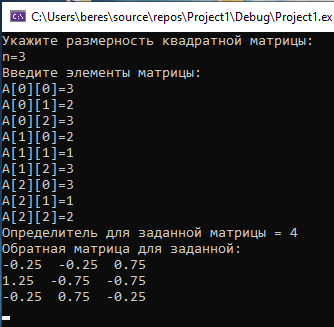
\includegraphics[width=0.7\textwidth]{Рисунок2.PNG}
	\caption{Окно программы с обратной матрицей}\label{fig:par}
\end{figure}

\end{document}
